%!TEX root = ../terrainbook.tex

\graphicspath{{runoff/}}


\nobibliography*


\chapter{Application: Runoff modelling}

Many interesting DTM operations are based on runoff modelling, \ie\ the computation of the flow and accumulation of water on a terrain.
Examples include: knowing where streams will form in the case of heavy rainfall, finding the areas that will be affected by a waterborne pollutant, tracing the areas that could become submerged by floodwater, or calculating the rate of erosion or sedimentation in a given area.

In hydrology, runoff modelling can be very complex (Figure~\ref{fig:hydrology}).
Hydrological models usually consider different precipitation scenarios, model various types of overland and subsurface flows, and take into account many location- and time-dependent factors, such as the depth of the water table and the permeability of the soil.
Such models can be quite accurate, but they require high-resolution data that is often not available, they are difficult to create without specialised knowledge, and they involve substantial manual work.

\begin{figure}[htbp]
\centering
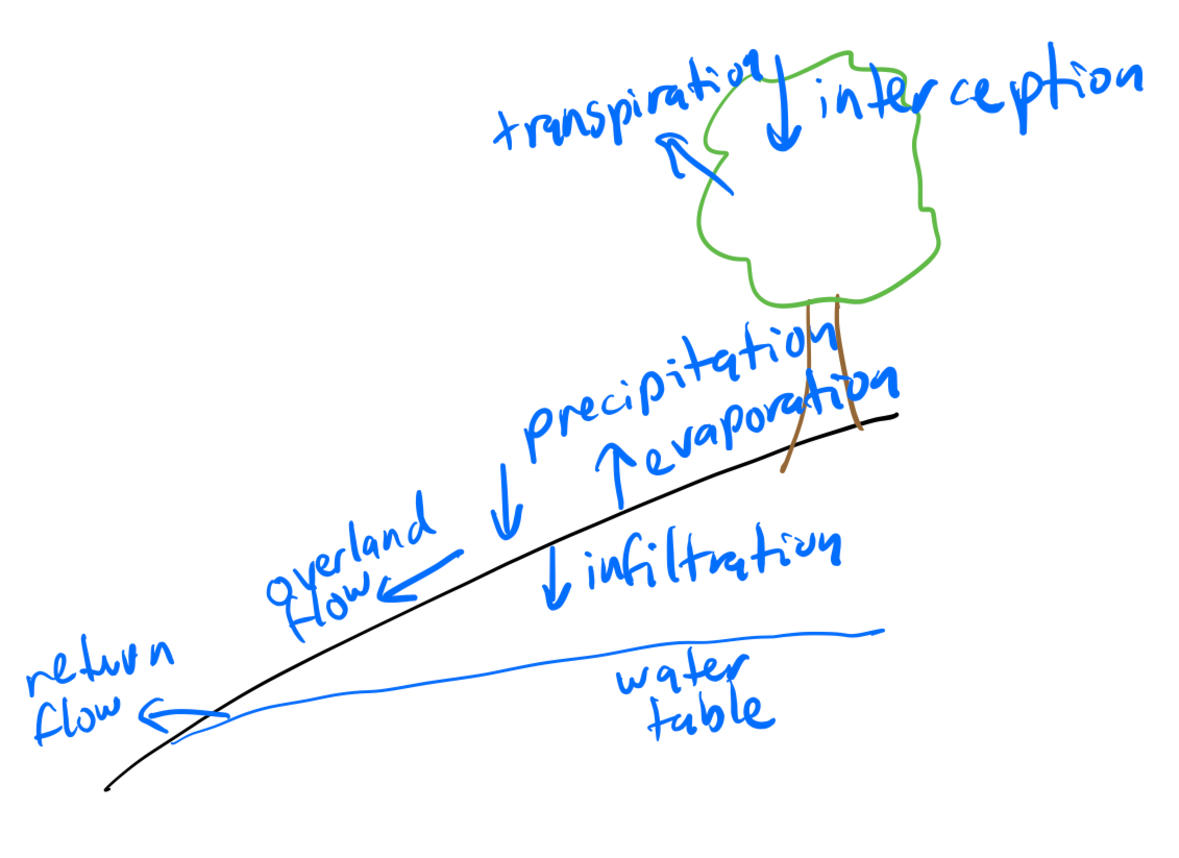
\includegraphics[width=0.75\linewidth]{figs/hydrology.pdf}
\caption{Different types of water flows as modelled in hydrology. Based on \citet{Beven12}.}%
\label{fig:hydrology}
\end{figure}

By contrast, the simpler GIS models of runoff can be performed automatically in large areas with only a DTM\@.
These models mostly use gridded raster terrains, and so we will generally refer to these in this chapter, but most methods work with other representations.
In order to achieve this, two big assumptions are usually made:

\begin{enumerate}
\item that all water flow is \emph{overland}, thus ignoring all subsurface flows and dismissing factors such as evaporation and infiltration; and
\item that a good estimate for the total flow at any point is the drainage area upstream from it, \ie\ the area above the point which drains to it, which is roughly equivalent to rain that is falling evenly all over a terrain.
\end{enumerate}

Based on these assumptions, runoff modelling is simplified by considering only two values, which are computed for every cell in a DTM\@:

\begin{description}
\item[Flow direction]
Given a DTM cell, towards which nearby cells and in which proportions does water flow from it?
\item[Flow accumulation]
Given a DTM cell, what is the total water flow that passes through it?
\end{description}

We look at a few different methods to compute these values in the next two sections.

\section{Computing the flow direction}%
\label{se:direction}

Theoretically, the flow direction of a point is the direction with the steepest descent at that location, which does correspond to the direction that water would naturally flow towards.
However, the discretisation of a terrain into DTM cells means that some kind of an approximation needs to be made.
There are two broad approaches that can be followed to do this: computing a single flow direction or multiple flow directions per DTM cell.

\subsection{Single flow direction}

% Perpendicular to contours in a 2D map

The earliest and simplest method to compute the flow direction of a cell is to compute the slope between the centre of the cell and the centre of all its neighbouring cells (using the distance between the centres and the difference in elevation), then assign the flow direction towards the neighbour with the steepest descent.
The method is known as the \emph{single flow direction (SFD)} approach, and when applied to a raster grid, where there are eight neighbours to each pixel (left, right, up, down and the diagonals), it is also known as the \emph{eight flow directions (D8)} approach.

On one hand, the method is very fast and easy to implement, and it avoids dispersing the water flow between multiple cells.
On the other hand, it can have significant errors in the flow direction, and it does not allow for divergent flows.
For instance, in a square grid, they can be of up to \(22.5^\circ{}\) (because the method is forced to choose a neighbouring cell in increments of \(45^\circ{}\)).
This method can therefore easily create artefacts in certain geometric configurations (Figure~\ref{fig:d8}).

Many of these artefacts can be eliminated by using the rho8 method, which modifies D8 to assign the flow direction to one of its lower neighbours randomly with probability proportional to the slope.
However, it produces non-deterministic results, which is often a sufficient reason not to use it.

Despite its limitations, the SFD method is still widely used and available in many GIS tools\@.

\begin{figure}[htbp]
\centering
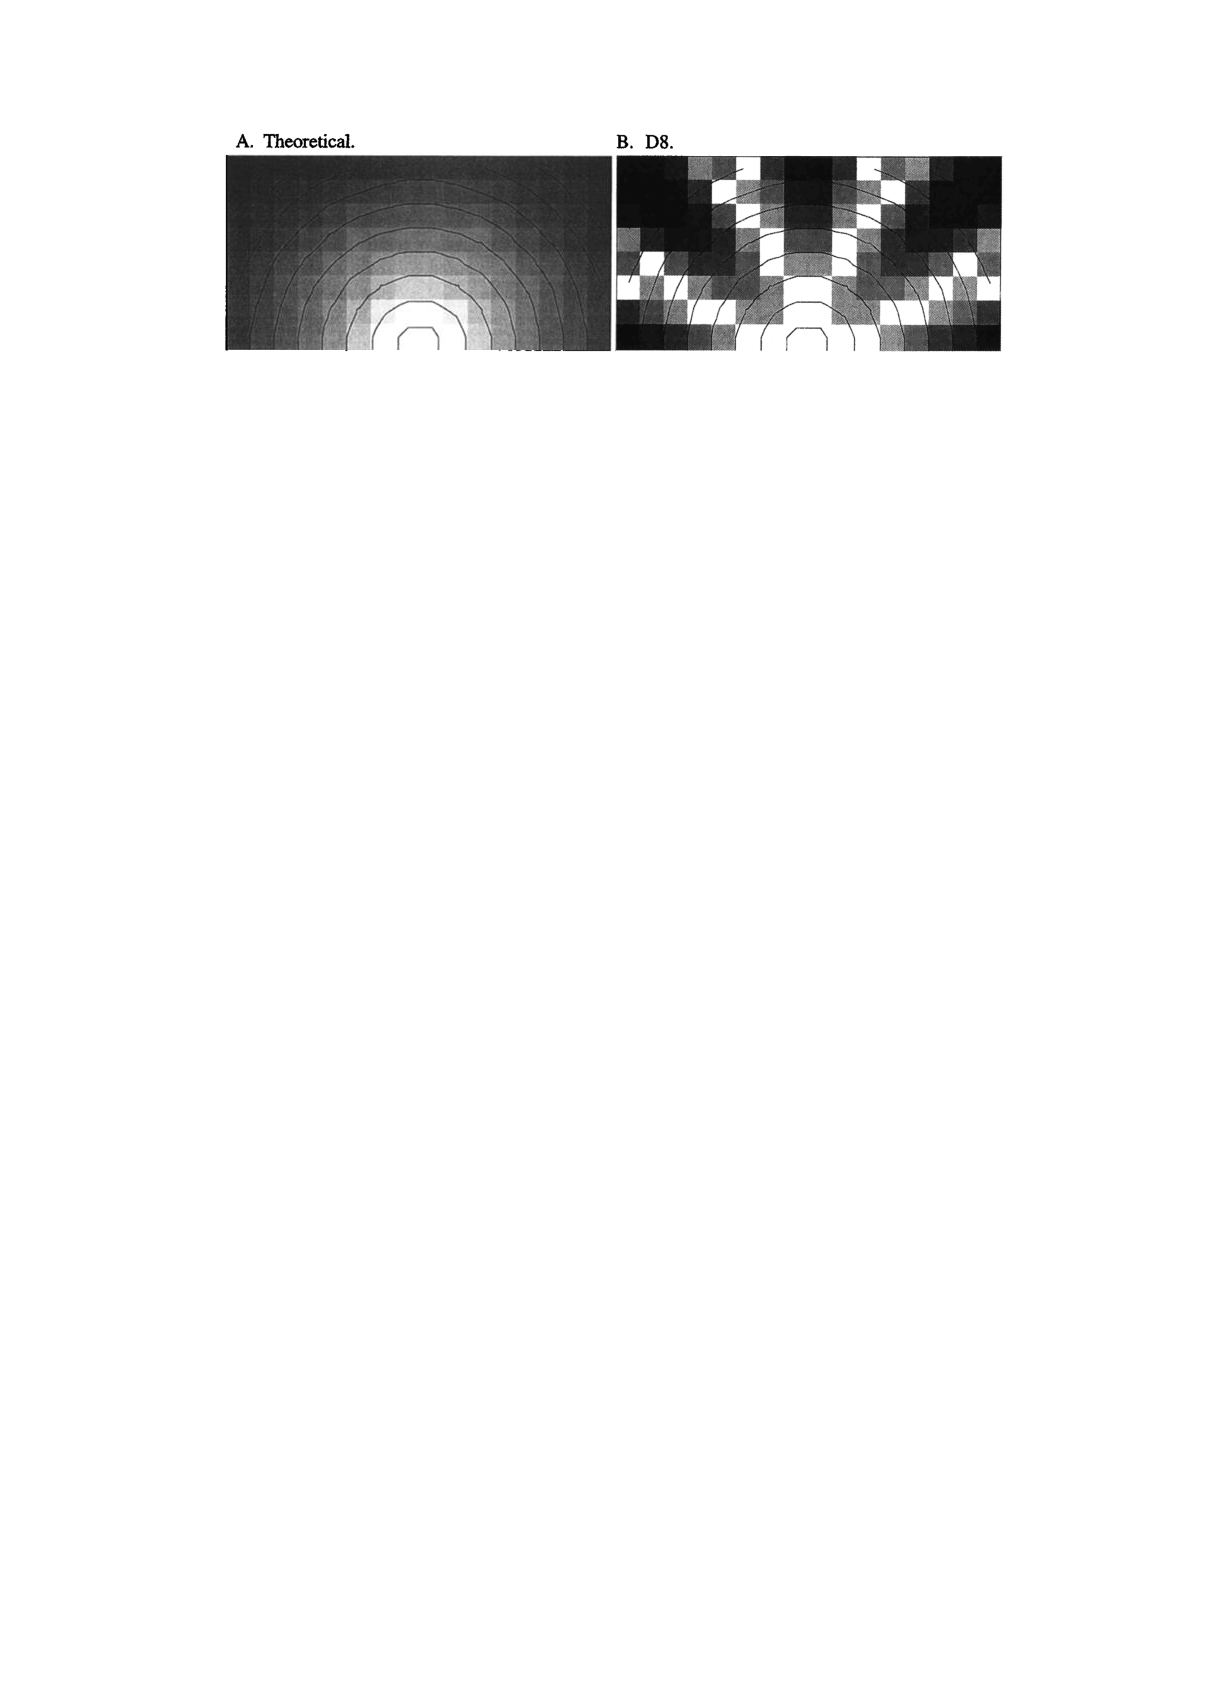
\includegraphics[width=0.75\linewidth]{figs/d8.pdf}
\caption{The D8 method creates artefacts when water is draining from a circular cone. From \citet{Tarborton97}.}%
\label{fig:d8}
\end{figure}

\subsection{Multiple flow directions}

In an attempt to overcome the limitations of the SFD method, a variety of methods assign the flow direction of a DTM cell fractionally to all of its lower neighbouring cells according to some criteria.
These methods are collectively known as multiple flow directions (MFD), and they usually look like:

\begin{equation}
F_i = \frac{\left(L_i \tan{\alpha_i}\right)^x}{\sum_{j=1}^{n}\left(L_j \tan{\alpha_j}\right)^x}
\end{equation}

where \(F_i\) is the flow towards the i-th neighbouring cell, \(L_i\) is the flow width (Figure~\ref{fig:quinn}), \(\alpha_i\) is the gradient towards the i-th neighbouring cell (and so \(\tan(\alpha_i)\) is the slope), \(x\) is an exponent that controls the dispersion, and \(n\) is the number of neighbours of the cell.

\begin{figure}[htbp]
\centering
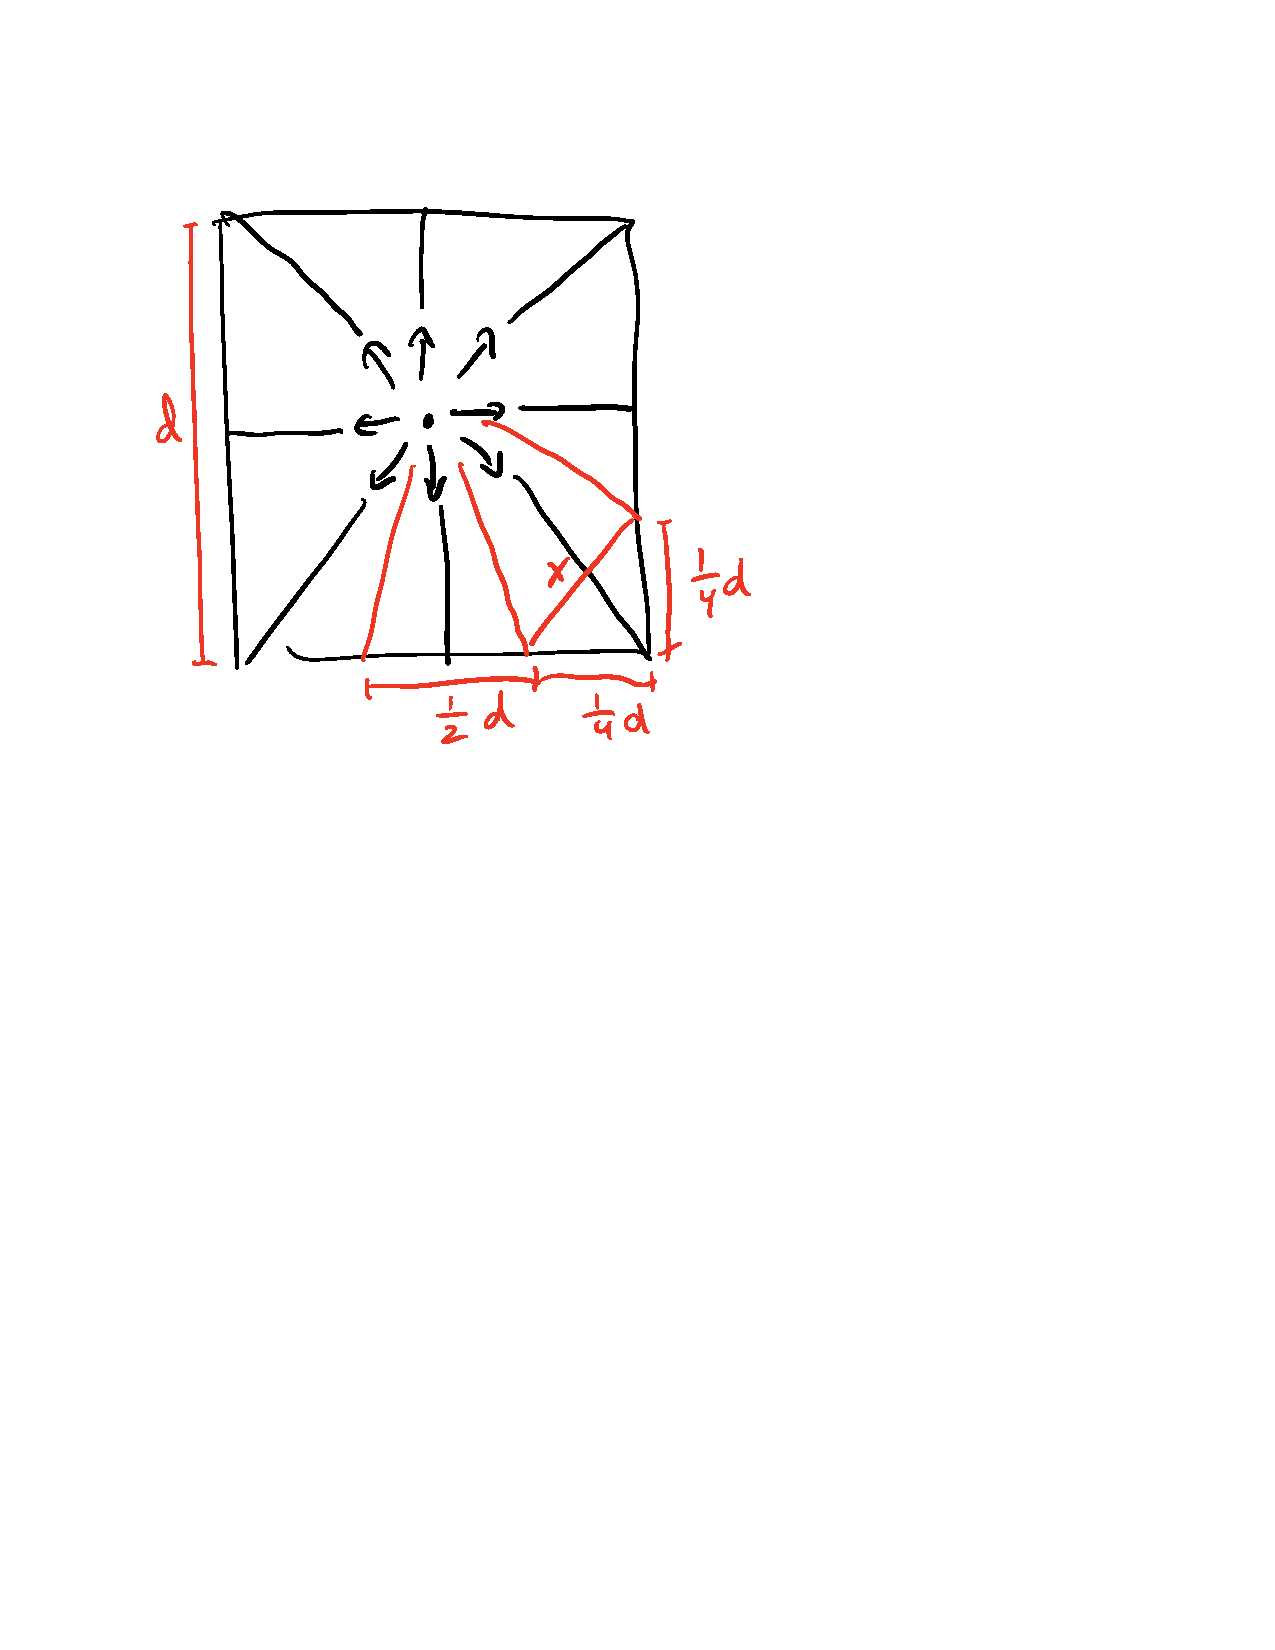
\includegraphics[width=0.5\linewidth]{figs/quinn.pdf}
\caption{The flow width \(L\) can be computed using the geometry of the DTM cells.
In the case of a square grid with spacing \(d\), it is \(\frac{\sqrt{2}}{4}d\) for the diagonals (\(L_2\)) and \(\frac{1}{2}d\) for the adjacencies (\(L_1\)), where \(d\) is the grid spacing. Based on \citet{Quinn91}.}%
\label{fig:quinn}
\end{figure}

\begin{link-box}
\paragraph{Look at Figures~4--9 in the following paper.} These show the results of using a few flow direction computation methods in different terrains.
Pay attention to how these differ from the theoretical values (if given), how some methods tend to create artefacts (\eg\ D8 in Figure~4), and how dispersion affects some others (\eg\ \citet{Quinn91} in Figure~7).
\\
\\
\bibentry{Tarborton97}\\
\textbf{PDF:} \url{https://doi.org/10.1029/96WR03137}
\end{link-box}

\section{Computing the flow accumulation}%
\label{se:accumulation}

After the flow directions in all the cells of a DTM have been computed, the usual next step is to use this information to compute the flow accumulation in all of them.
As stated in the assumptions we make for GIS models of runoff, the flow accumulation at a given DTM cell can be estimated by the area that drains to it.
Note that in the case of a square grid, it is simply the number of cells that drain to it.

In practical terms, the flow accumulation is usually computed with a recursive operation:

\begin{equation}
A_0 = a_0 + \sum_{i=1}^{n} p_i A_i
\end{equation}

where \(A_0\) is the accumulated flow for a cell, \(a_0\) is the area of the cell, \(p\) is the proportion of the i-th neighbour that drains to the cell, \(A_i\) is the accumulated flow for the i-th neighbour, \(n\) is the total number of the neighbouring cells.
Note that this calculation can be sped up substantially by: (i) storing the accumulated flows that have already been computed, and (ii) not following the recursion when \(p_i = 0\).

\section{Solving issues with sinks}

Sinks, which are also known as depressions or pits, are areas in a DTM that are completely surrounded by higher terrain.
Some of these are natural features that are present in the terrain (\eg\ lakes and dry lakebeds) and where water would flow towards in reality, and are thus not a problem for runoff modelling.
However, they can also be artefacts of the DTM (\eg\ noise and areas without vegetation can create depressions) or very small and easily flooded\@, in which case we need to implement a mechanism to route water flows out of these depressions.
We will look at two common options to solve this problem: modifying a DTM by filling in (certain) sinks, and implementing a flow routing algorithm that allows water to flow out of sinks.

\subsection{Filling in sinks}

The aim of the algorithms to fill in sinks is to increase the elevation of certain DTM cells in a way that ensures that all the cells in the DTM can drain to a cell on its boundary (or possibly to a set of cells that are known to be valid outlets, \eg\ lakes and oceans)\@.
At the same time, the elevation increases should be minimised in order to preserve the original DTM as much as possible.

\begin{link-box}
\textbf{Section~3 in the following paper.} It explains the priority-flood algorithm, which is an efficient method to fill in sinks.
In short, it keeps a sorted list of DTM cells that are known to drain to the boundary (and possibly other cells that are known to drain), which is initialised with the cells on the boundary of the DTM (and possibly other cells)\@.
Then, it iteratively: (i) removes the lowest cell from this list, (ii) increases the elevation of its neighbours that are not yet known to drain to the level of the cell, (iii) adds the neighbours that are not yet known to drain to the list.
\\
\\
\bibentry{Barnes14a}\\
\textbf{PDF:} \url{https://doi.org/10.1016/j.cageo.2013.04.024}
\end{link-box}

\subsection{Least-cost (drainage) paths}

An alternative to modifying a DTM to eliminate sinks is to implement a more complex water routing algorithm that allows water to flow out of sinks.
For this, the usual approach is to implement a variation of the \(A^{*}\) search algorithm, which in this context is known as the least-cost paths (LCP) algorithm.

\begin{link-box}
\textbf{Section~2.1 in the following paper.} It explains the LCP algorithm and how it is implemented in GRASS\@.
In short, it keeps a sorted list of DTM cells that are known to drain to the boundary (and possibly other cells that are known to drain), which is initialised with the cells on the boundary of the DTM (and possibly other cells)\@.
Then, it iteratively: (i) removes the lowest cell from this list, (ii) sets the drainage direction of its neighbours that are not yet known to drain towards itself, (iii) adds the neighbours that are not yet known to drain to the list.
Note the similarity with the algorithm in \citet{Barnes14a}.
\\
\\
\bibentry{Metz11}\\
\textbf{PDF:} \url{https://doi.org/10.5194/hess-15-667-2011}
\end{link-box}

\section{Assigning flow direction in flats}

Flats are areas in a DTM that have the same elevation.
They therefore do not have a well-defined flow direction, which causes problems for many water routing algorithms.
Flats can sometimes occur naturally, but they are more often the result of precision limits, noise removal, or sink filling algorithms.

It is thus often necessary to apply a method that assigns a flow direction to flats, either by: (i) modifying the DTM to eliminate them, and then assigning them a flow direction in the usual way, or (ii) assigning them a flow direction directly.

\begin{link-box}
\textbf{Section~2 in the following paper.} 
It describes an algorithm to directly assign a flow direction to flats using a combination of: (i) a gradient away from higher terrain (\ie\ terrain goes down as we move away from higher terrain), and (ii) a gradient towards lower terrain (\ie\ terrain goes down as we move closer to lower terrain).
\\
\\
\bibentry{Barnes14}\\
\textbf{PDF:} \url{https://doi.org/10.1016/j.cageo.2013.01.009}
\end{link-box}

\section{Drainage networks and basins}

Interpreting DTM cells as nodes and the flow direction as directed edges connecting them yields the \emph{drainage network} of a DTM\@.
However, it is usually best to filter out the least important parts of the network using a flow accumulation threshold.
A good rule of thumb for this threshold is the mean flow accumulation in the DTM, but an exact value is usually set by trial and error until the desired parts of the network are kept.

Based on a computed drainage network, it is then possible to extract the \emph{drainage basins} of a DTM by considering the areas that are drained by one or more nodes of the network (Figure~\ref{fig:oceans}).
This operation can be performed in many different places, such as the end node of a river (yielding its river basin), the nodes just before junctions in the network (yielding the drainage basins of the tributaries of a river), or the end nodes of a selected part of the network (yielding the drainage basin of a sea or ocean).
The lines that separate adjacent drainage basins are \emph{drainage divides}, which form topographical ridges.

\begin{figure}[htbp]
\centering
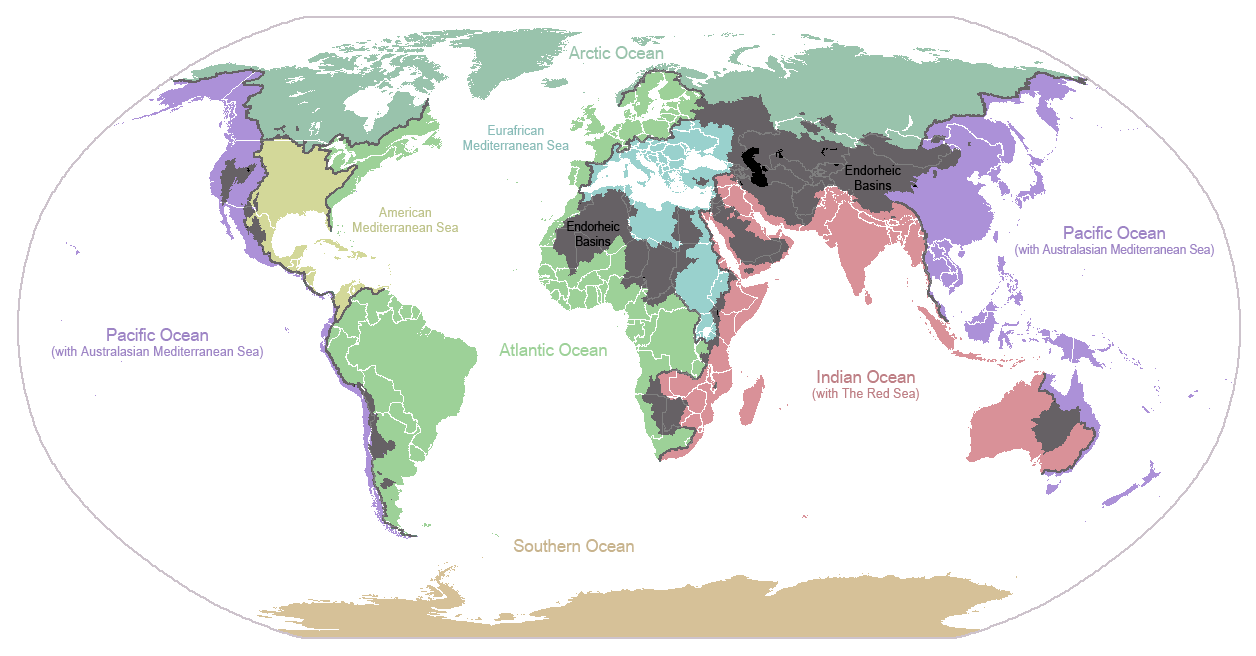
\includegraphics[width=\linewidth]{figs/Ocean_drainage}
\caption{The areas that drain to all the oceans can be computed by selecting the DTM cells on the coastline of these oceans and finding the areas that drain through them.
Note the endorheic basins that drain to none of these cells.
These actually form sinks in the DTM\@.
From Wikimedia Commons.}%
\label{fig:oceans}
\end{figure}

%%%
%
\section{Notes and comments}

\citet{Beven12} is a good reference book on hydrology.
It covers how to make much more complex runoff models than the ones described here.

\citet{OCallaghan84} was the original paper to describe the D8 method.
\citet{Fairfield91} modify D8 into the stochastic rho8 method.
\citet{Quinn91} describes the original MFD method.
\citet{Tarborton97} describes the alternative (D\(^{\infty}\)) MFD method and contains nice figures comparing multiple methods.

\citet{Barnes14a} describes how to fill in sinks, while \citet{Metz11} describes how to use a variation of \(A^{*}\) search algorithm to route water out of them.
\citet{Barnes14} describes how to assign the drainage direction over flats.


